\section{Simulation of e-beam exposed PMMA viscosity profile}
In this study, thermal reflow is simulated for PMMA with non-uniform viscosity profile caused by e-beam exposure at room temperature.
According to equations~\ref{eq:WLF} and \ref{eq:3p4_3p1}, one can calculate PMMA viscosity for any specific temperature and number average molecular weight, so PMMA number average molecular weight distribution is of interest.
The distribution of PMMA local $M_n$ could be obtained by simulation of e-beam induced PMMA main-chain scissions.
For the latter, Monte-Carlo simulation of e-beam scattering in PMMA/Si structure was implemented.
Elastic scattering cross-section were obtained by relativistic partial wave expansion method (Mott cross-sections) using free software ``ELSEPA''~\cite{ELSEPA}.
Inelastic scattering was simulated using models based on energy loss functions of PMMA and Si, provided by Dapor~\cite{Dapor} and Valentin~\cite{Valentin}.
Next, according to Aktary~\cite{Aktary}, PMMA main-chain scissions were supposed occur due to inelastic electron-electron scattering.
Electron-electron scattering events, leading to PMMA main-chain scissions were simulated by Monte-Carlo technique with introducing the scission probability ($p_s$):
\begin{equation}
	\mathrm{electron-electron \ inelastic \ scattering: \ } \cases{\xi < p_s: & scission \\
		\xi \geq p_s: & no scission}
\end{equation}
where $\xi$ -- a random variable uniformly distributed on [0, 1).
Value of $p_s$ for room temperature (25 $^\circ$C) was determined by simulation of experimental radiation scission yield using the approach described in our previous paper~\cite{my_MEE} and compised 0.05.

Simulated PMMA main-chain scission events were stored in 3D histograms with 50~nm bin size.
The example of PMMA main-chain scission distribution simulated for line exposure using this approach is shown in Fig.~\ref{fig:sci_hist}.

\begin{figure}[h]
	\centering
	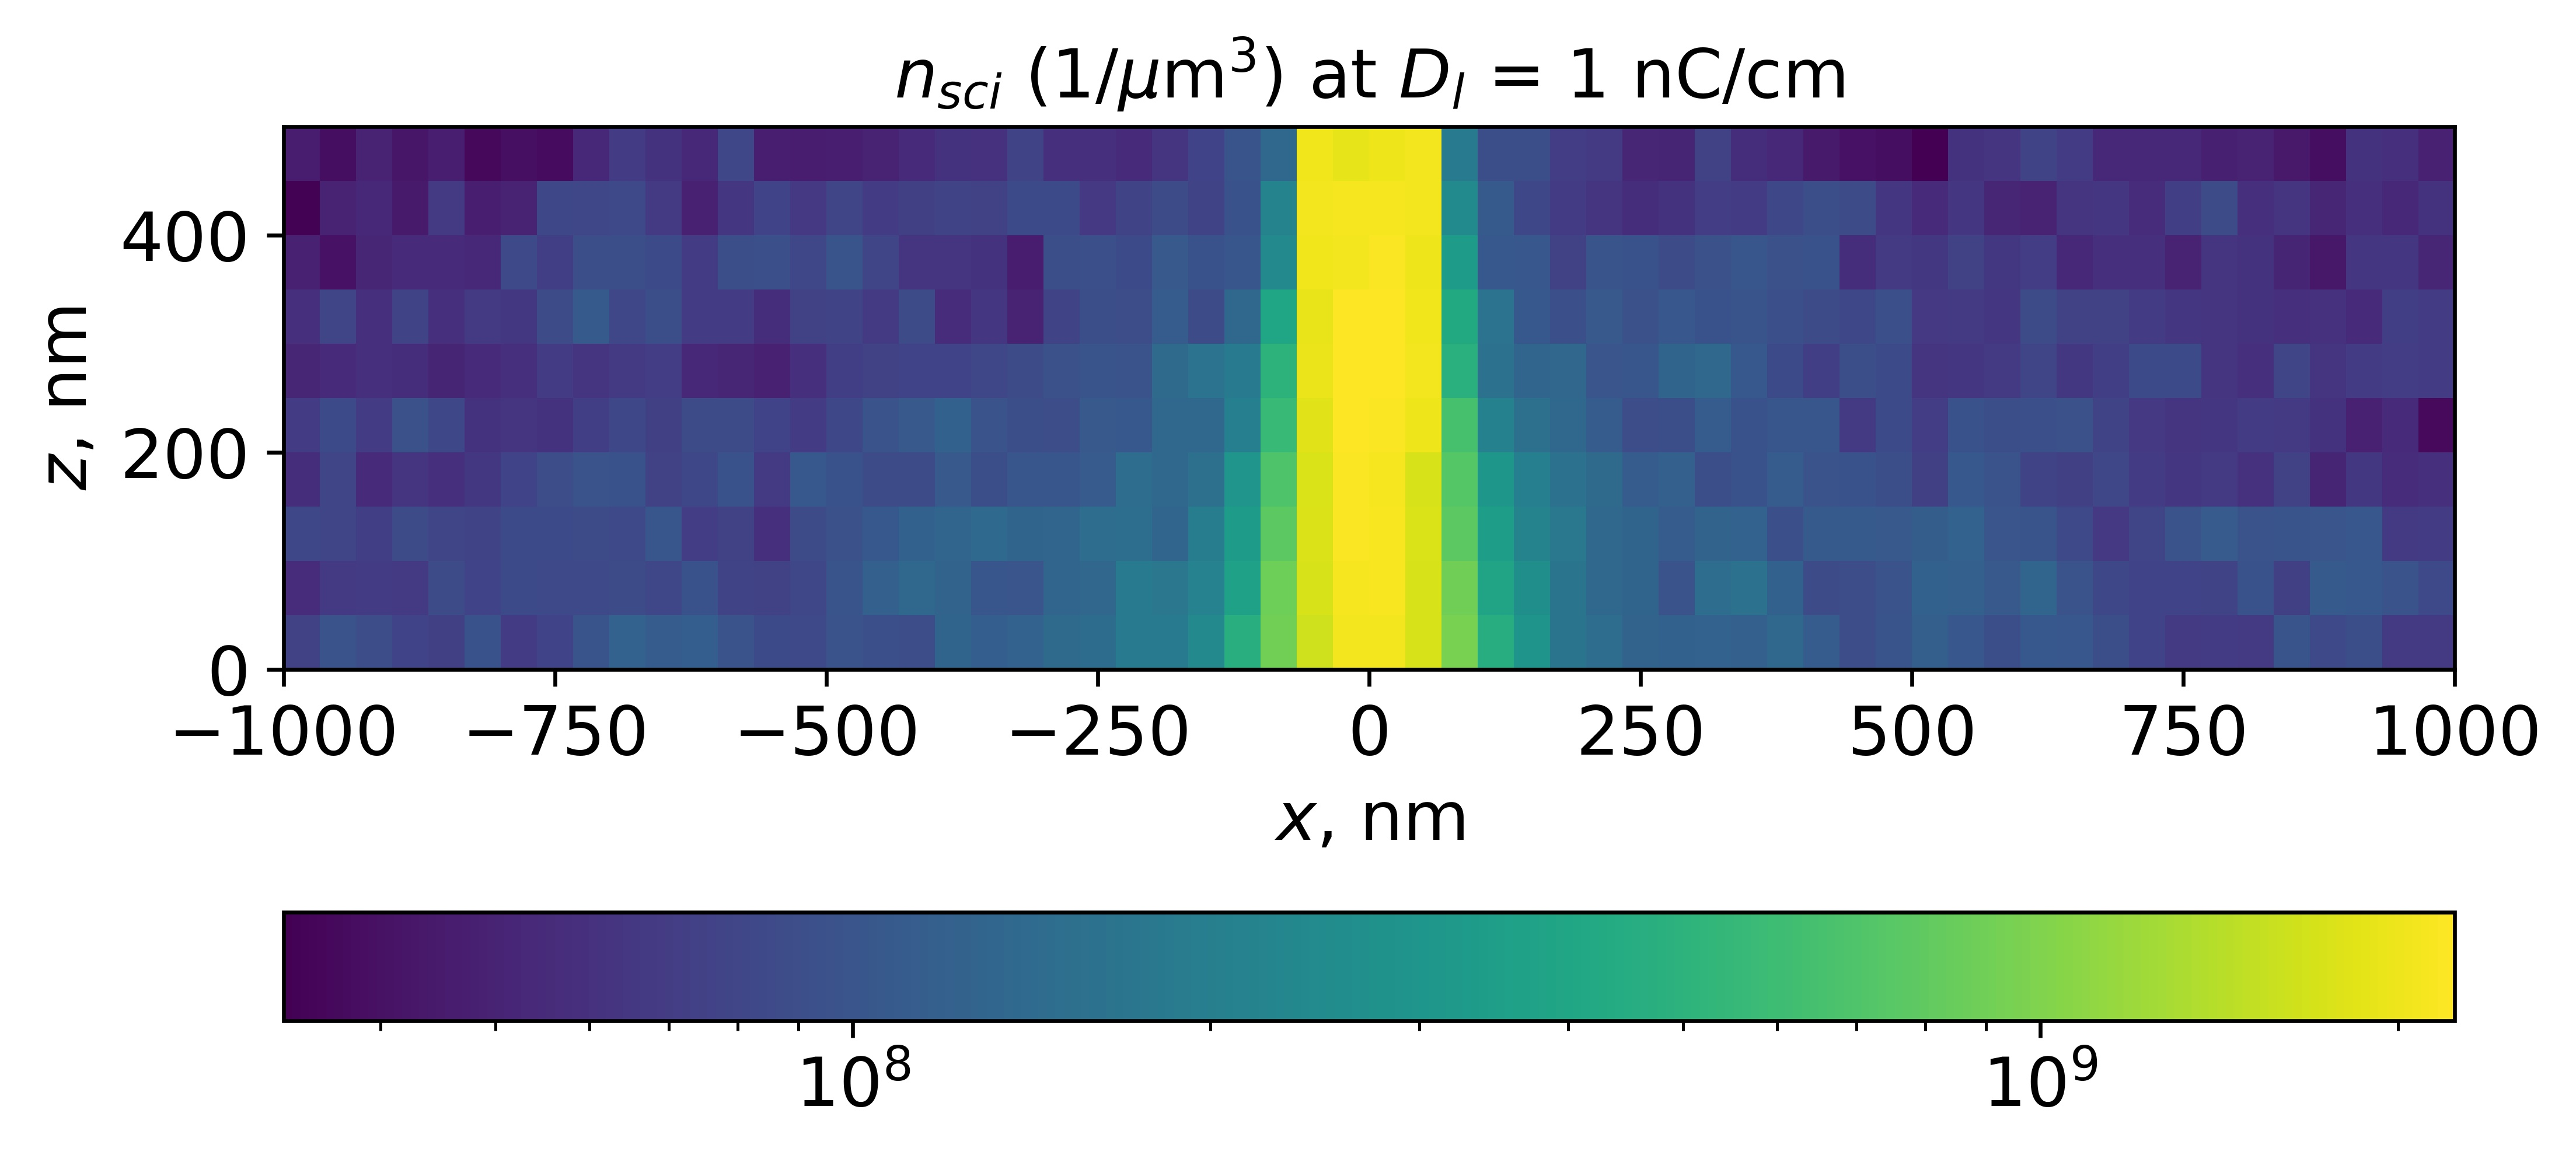
\includegraphics[width=0.8\linewidth]{sci_conc_1uC_cm_LOG}
	\caption{
		Simulation of local PMMA main-chain scission concentration in PMMA layer for line exposure.
		Line dose is 1 nC/cm, line width -- 300~nm, e-beam energy -- 20 keV, PMMA layer thickness -- 500 nm.
		Scission probability in inelastic electron-electron scattering is 0.05, which corresponds to room temperature (25$^\circ$C).
	}
	\label{fig:sci_hist}
\end{figure}

Then, number average molecular weight was calculated for each bin using the model of scissions randomly occurring at the bonds between the monomers~\cite{Ku1969}:
\begin{equation}
	\frac{1}{M_n^\prime} = \frac{w_s}{M_0} + \frac{1}{M_n},
\end{equation}
where $M_n$ and $M_n^\prime$ -- PMMA number average molecular weight before and after exposure, respectively, $M_0$ -- monomer molecular weight (100 for methyl methacrylate, MMA), $w_s$ -- probability of scission at a bond.
$w_s$ values were calculated for each bin using the formula:
\begin{equation}
	w_s = \frac{N_{sci}}{N_{mon}},
\end{equation}
where $N_{sci}$ -- number of scissions and $N_{mon}$ -- number of monomers in the bin, respectively.
Number of monomers in the bin of (50~nm)$^3$ size was calculated from PMMA density (1.19 g/cm$^3$) and MMA molecular weight (100 g/mol) and comprised 894809.
The example of $M_n^\prime$ distribution, simulated for line exposure by this method, is shown in Fig.~\ref{fig:Mn_hist}.

\begin{figure}
	\centering
	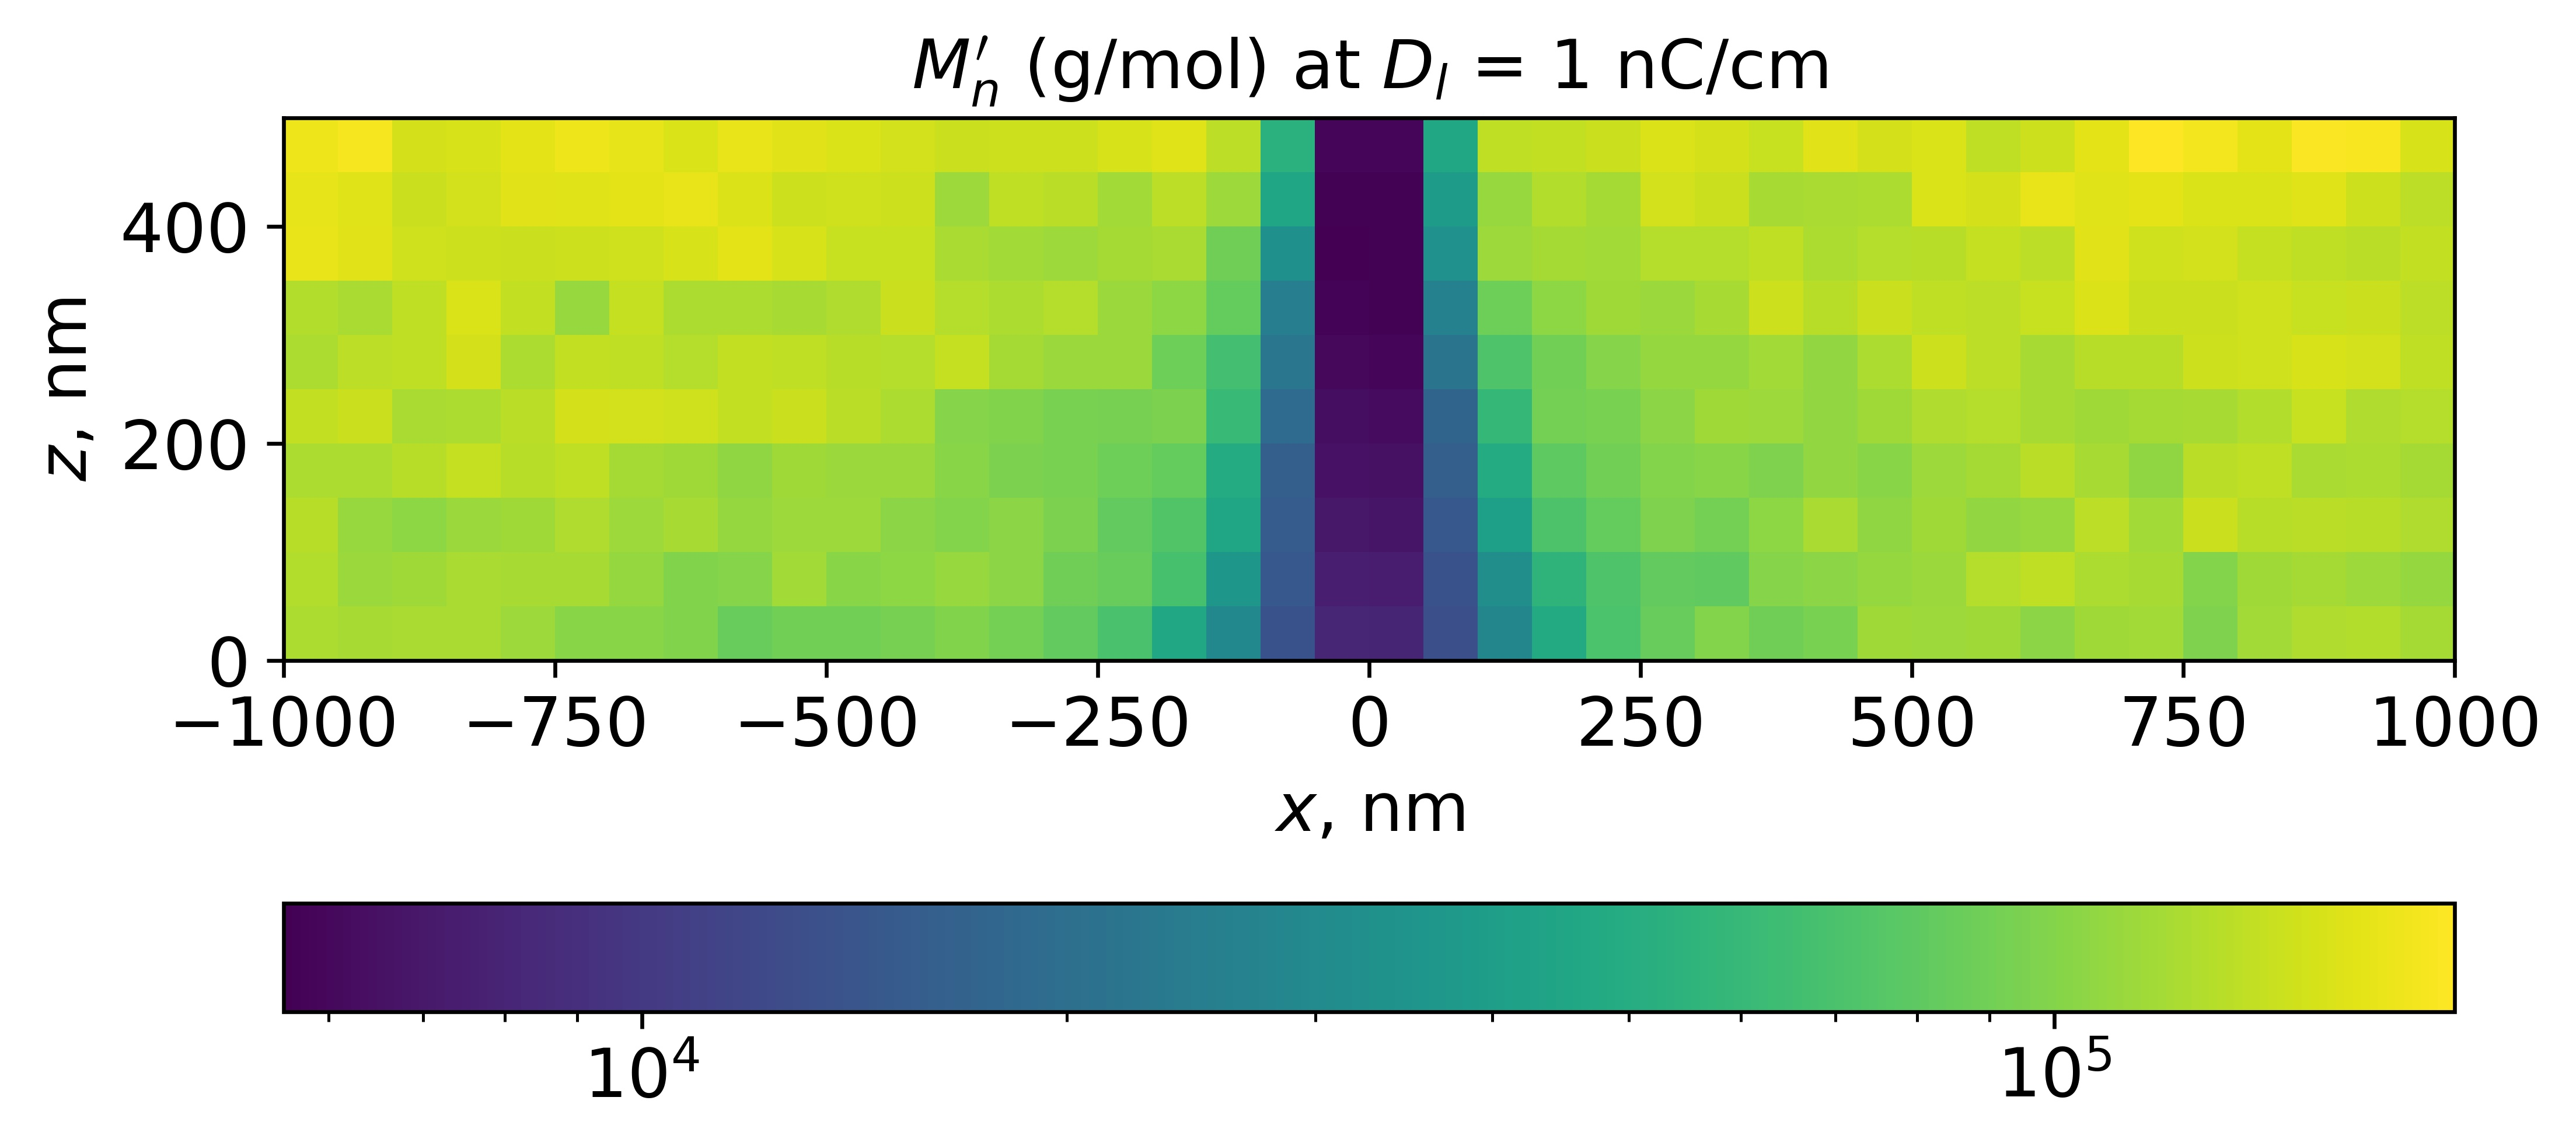
\includegraphics[width=0.8\linewidth]{Mn_prime_mat_easy_1_nC_cm_LOG}
	\caption{
		Simulation of local number average PMMA molecular weight in PMMA layer for line exposure at room temperature.
		Line dose is 1 nC/cm, line width -- 300~nm, e-beam energy -- 20 keV, PMMA layer thickness -- 500 nm.
		Initial PMMA number average molecular weight is 271000.
	}
	\label{fig:Mn_hist}
\end{figure}

Finally, local viscosity of exposed PMMA was calculated for required temperature using equation~\ref{eq:WLF} and for the following simulation viscosity distribution is averaged along $z$ axis (Fig.~\ref{fig:eta_arr}).

\begin{figure}
	\centering
	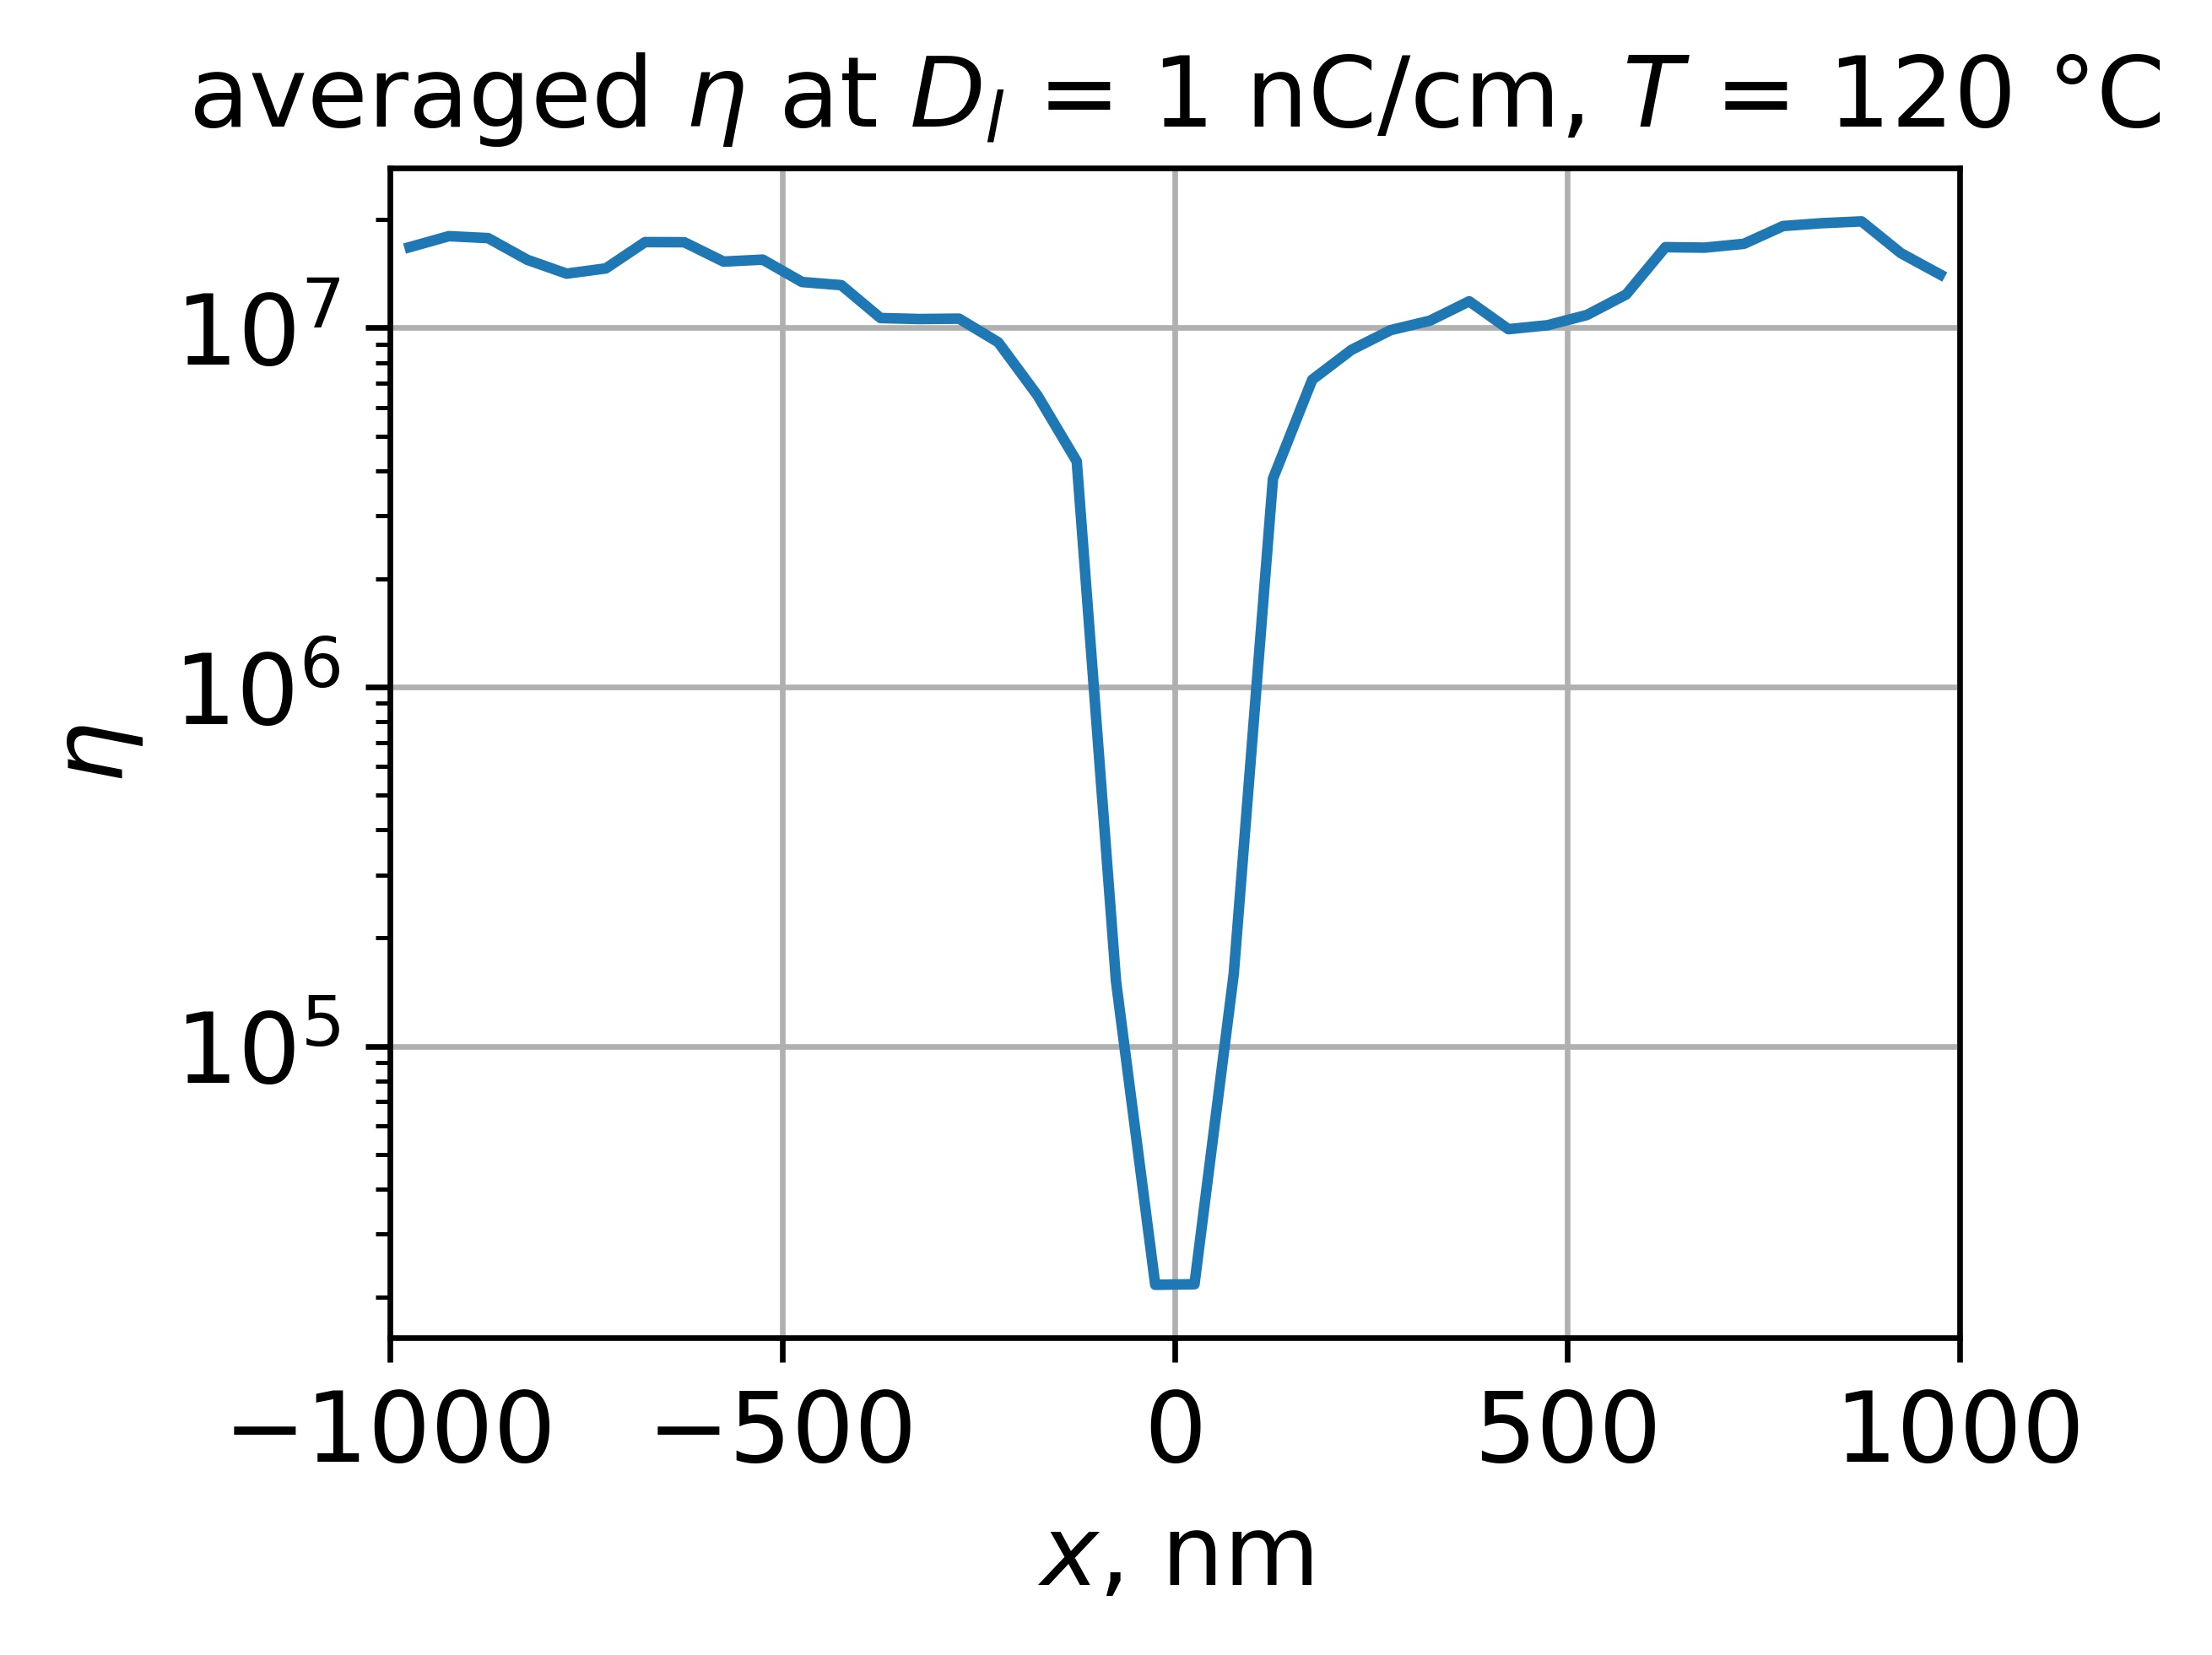
\includegraphics[width=0.6\linewidth]{eta_arr_1_nC_cm_120C_LOG}
	\caption{
			Simulation of averaged (along $z$ axis) viscosity profile in e-beam exposed PMMA layer for 120 $^\circ$C.
			Line dose is 1 nC/cm, e-beam energy -- 20 keV, PMMA layer thickness -- 500 nm.
			Initial PMMA number average molecular weight is 271000, PMMA reflow temperature is 120~$^\circ$C.
		}
	\label{fig:eta_arr}
\end{figure}
